\subsection{Propensity updating}
\label{sec:reaction_update}

In \refsect{sec:reaction_selection}, we have introduced methods to perform a multinomial drawing among $N$ propensity values.
We have seen that special structures can improve the drawing time
but there is an additional cost to update those structures when a propensity value changes.
Here we will study how this additional cost evolves
when $U$ propensities need to be changed from one drawing to the next drawing.

\subsubsection{Naive method: why not update everything?}

We begin with the simple case where $U = N$.

\paragraph{Direct Method}
In the direct method, we need to compute the total propensity of the system,
so we need to loop through all propensities at least once.
In this sense, the overall update complexity is $O(N)$ and the total complexity (including drawing) is equally $O(N)$.

\paragraph{Binary Tree}
We need to update all leaves of the tree.
Naively, this would lead to a $O(N\log N)$ overall update complexity.
However, this assumes that each time a leaf value is updated, we update all the intermediate nodes up to the root.
In practice, it is possible to differ update of intermediate nodes and just mark them as outdated.
We only update them once all their children have been treated,
so that every node is updated at most once.
In the case where all leaves are updated, every node in the tree is updated exactly once.
The complexity is thus given by the number of nodes in the tree, approximately $2N$,
yielding $O(N)$ overall update complexity.
The total complexity is then $O(\log N + N) = O(N)$.

\paragraph{Hybrid Method}
Here the update algorithm is applied to every propensity, yielding a overall $O(N)$ update complexity.
Total complexity is $O(1 + N) = O(N)$.

\paragraph{Summary}
As a matter of fact, when propensities are updated naively,
the benefit of using sophisticated structures is (asymptotically) lost~\reftabp{tab:naive_update}.
\begin{table}[!h]
  \centering
  \begin{tabular}{|l|c|c|c|}
    \hline
    Method & Drawing Complexity & Update Complexity & Total Complexity\\
    \hline
    Direct Method & $O(N)$ & $O(N)$ & $O(N)$\\
    Binary Tree & $O(\log N)$ & $O(N)$ & $O(N)$\\
    Hybrid Method & $O(1)$ & $O(N)$ & $O(N)$\\
    \hline
  \end{tabular}
  \caption{Worst-case complexities for $U=N$.}
  \label{tab:naive_update}
\end{table}

It is absolutely necessary to keep $U$ as small as possible.
Formally, we need to determine a subset of propensities that includes all propensities that might have changed.
In that case, specific drawing structures start to be interesting~\reftabp{tab:general_update}.
Roughly speaking, the binary tree is better than the direct method as soon as $U < N / \log N$
and the hybrid method outcompetes the two other methods for $U < N$.

This trend is even stronger in a system where the number of propensities to update does not depend on $N$~\reftabp{tab:ideal_update}.
In this case, the direct method is linear, the binary tree logarithmic and the hybrid method constant time,
yielding huge improvements when switching from one method to the next one.

\begin{table}[!h]
  \centering
  \begin{tabular}{|l|c|c|c|}
    \hline
    Method & Drawing Complexity & Update Complexity & Total Complexity\\
    \hline
    Direct Method & $O(N)$ & $O(U)$ & $O(N)$\\
    Binary Tree & $O(\log N)$ & $O(\min\{U\log N,N\})$
    & $O(\min\{U\log N,N\})$\\
    Hybrid Method & $O(1)$ & $O(U)$ & $O(U)$\\
    \hline
  \end{tabular}
  \caption{Worst-case complexities for a general $U \leq N$.}
\label{tab:general_update}
\end{table}

\begin{table}[!h]
  \centering
  \begin{tabular}{|l|c|c|c|}
    \hline
    Method & Drawing Complexity & Update Complexity & Total Complexity\\
    \hline
    Direct Method & $O(N)$ & $O(1)$ & $O(N)$\\
    Binary Tree & $O(\log N)$ & $O(\log N)$ & $O(\log N)$\\
    Hybrid Method & $O(1)$ & $O(1)$ & $O(1)$\\
    \hline
  \end{tabular}
  \caption{Worst-case complexities for the ideal case $U=O(1)$ (number of propensities to update does not scale with the number of reactions $N$ in the system).}
\label{tab:ideal_update}
\end{table}

\subsubsection{Using graphs to update propensities}

The most standard way to study how reactions influence each other is to draw a graph that tracks the dependencies between reactions.
A first version can be drawn using a \emph{bipartite graph} with reactions on one side and reactants on the other one.
We can draw two sets of vertices~\reffigp{fig:reactant_reaction_graph}.
\begin{itemize}
  \item If the reaction modifies the concentration of a reactant,
  a directed vertex is drawn from the reaction to the reactant.
  \item If the concentration of a reactant is used to compute the propensity of a reaction,
  a directed vertex is drawn that goes from the reactant to the reaction.
\end{itemize}

\begin{figure}[!h]
  \centering
  \begin{minipage}{0.39\textwidth}
    \[
    \begin{array}{l}
      R_1:\reactionIrr{A}{C+D}{}{} \\
      R_2:\reactionRev{B+C}{E}{}{} \\
      R_3:\reactionIrr{B+E}{2A}{}{} \\
      R_4:\reactionIrr{D+A}{B+A}{}{}
    \end{array}
    \]
  \end{minipage}
  \begin{minipage}{0.59\textwidth}
    \includegraphics[width=\textwidth]{graphs}
  \end{minipage}
  \caption{(Left) Sample reaction system.
  (Right) Corresponding bipartite graph displaying interactions between reactions and reactants.
  The reaction nodes were duplicated for readability.}
\label{fig:reactant_reaction_graph}
\end{figure}

\paragraph{Reactant to reaction graph}
The first algorithm we propose only takes advantage of the set of vertices that goes from reactants to reactions.
Here is the sketch of the algorithm:
\begin{itemize}
  \item We set up an \emph{observer pattern} to track changes in concentrations.
  Schematically, every time the concentration of a reactant changes,
  the reactant sends an update that will \emph{invalidate} the propensities in which it is involved
  (as pointed by the vertices on the graph).
  \item We initialize the system by computing all propensities.
  \item Until some target is reached:
    \begin{itemize}
      \item A random reaction is performed. Concentration of some reactant changes.
      Updates are sent and some propensities are invalidated.
      \item We recompute the propensities that were invalidated.
    \end{itemize}
\end{itemize}

\paragraph{Reaction to reaction graph}
In the second algorithm, we collapse the bipartite graph shown above into a graph that only contains reactions.
The collapsing process is rather intuitive if we use the directed vertices defined above.
Take two reactions $A$ and $B$.
There is a vertex $A \rightarrow B$ if there is some reactant $R$ such that $A \rightarrow R$ and $R \rightarrow B$ in the bipartite graph.
Put into words: when reaction $A$ occurs,
it changes the concentration of a reactant $R$ used to compute the propensity of $B$~\reffigp{fig:reaction_reaction_graph}.

\begin{figure}[!ht]
  \centering
  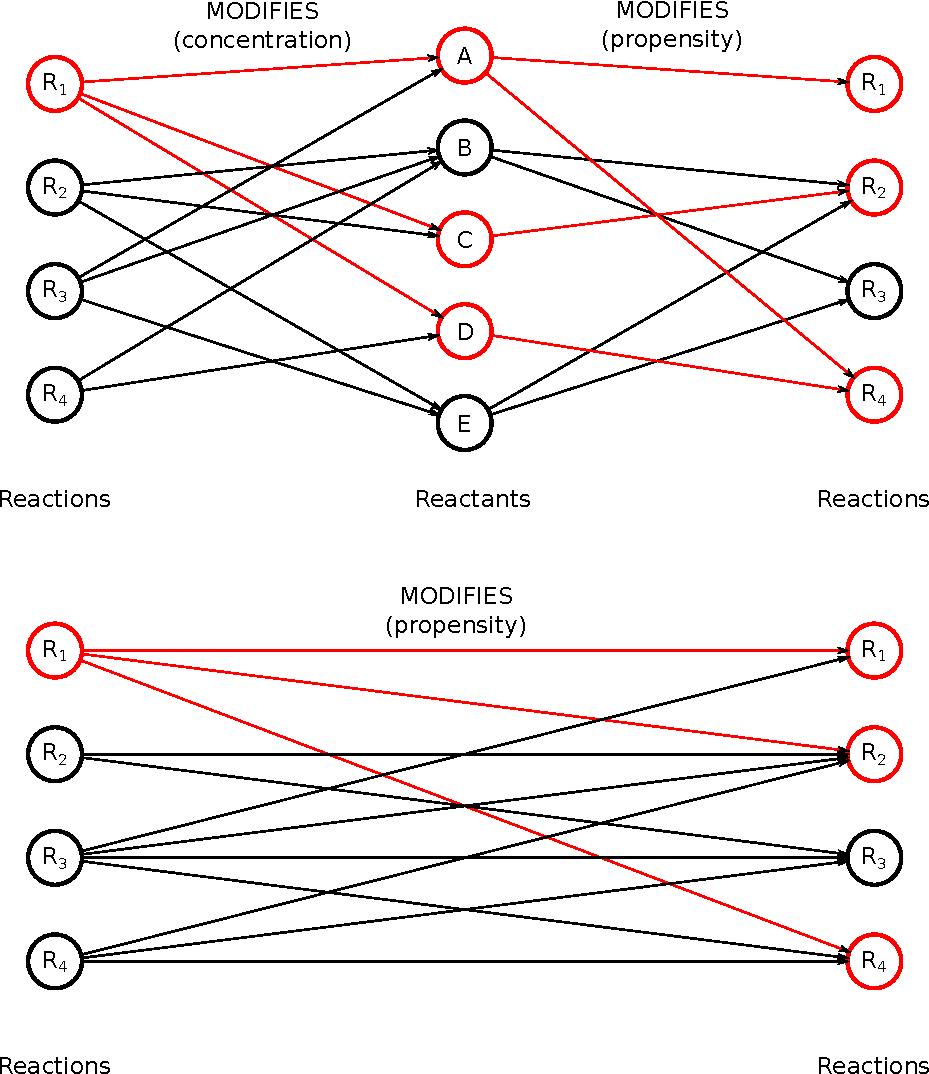
\includegraphics[width=0.6\textwidth]{graph_reaction_reaction}
  \caption{Collapsing bipartite graph into a pure reaction graph.
  (Top) Example of collapsing for reaction $R_1$.
  All paths leading to a potential propensity change in other reactions are displayed in red.
  (Bottom) Reaction to reaction graph.
  In red are the vertices that correspond to the paths displayed in red in the bipartite graph.
  Reaction nodes were duplicated for readability, the graph could also be represented with only one node for each reaction.}
\label{fig:reaction_reaction_graph}
\end{figure}

Here is a sketch of the algorithm:
\begin{itemize}
  \item We create the reaction graph:
  for each reaction we store the list of propensities to update when it occurs.
  \item We initialize the system by computing all propensities.
  \item Until some target is reached:
    \begin{itemize}
      \item A random reaction is performed.
      \item We recompute the propensities according to the reaction graph.
    \end{itemize}
\end{itemize}


\subsubsection{Pros and cons of graph algorithms}

\paragraph{Simple system}
The main difference between the algorithms is that the reactant to reaction algorithm uses an observer pattern.
This pattern it slightly more complicated to implement than the reaction graph.
Moreover, in closed systems of chemical reactions, the reaction graph approach is more efficient.
We can perform a very simple cost analysis for the update occurring after one reaction has been performed.
\begin{itemize}
  \item Rectant to reaction graph: for every reactant involved in the reaction, an update is sent that invalidates a subset of propensities.
  The subsets invalidated by the reactants might overlap, resulting in invalidating the same propensity several times.
  Note that invalidating does not mean recomputing the propensity,
  it is only recomputed after the whole invalidation process if it has been tagged by at least one reactant.
  \item Reaction to reaction graph: when the reaction occurs, we have direct access to the subset of propensities to recompute.
\end{itemize}

We see that there are additional costs in the reactant to reaction method
because of the update sending and possible overlaps that are eliminated
when the reactant to reaction graph is collapsed into the simpler reaction graph.
Depending on the system, these additional costs may not be negligible, even though they should remain fairly low.

\paragraph{System with external constraints}
If something else than a reaction might change the concentration of a reactant,
propensities will be updated correctly only when using the reactant to reaction algorithm.
When using the reaction graph, such interactions are not visible and
it may be necessary to update all propensities every time such an event occurs.

This flexibility problem can be overcome without an observer pattern
by storing both the reaction graph \emph{and} the bipartite graph to use the reactant to reaction graph when needed.
However, the solver still needs to be notified every time the concentration of a reactant changes due to external reasons.
There is a danger that this notification might be omitted by the programmer,
while an observer pattern guarantees that the solver will be aware of such changes.

\paragraph{System containing aggregated reactions}
In more complex systems that do not only include chemical reactions,
it is possible to include reactions that have multiple outcomes.
We developed a simulator that includes a \texttt{Loading} reaction.
A typical example is a RNA polymerase building a RNA by matching either
an ATP, a CTP, a GTP or a UTP depending on the DNA base it is reading.
The base is read dynamically during simulation,
so we do no know in advance which NTP pool is going to be impacted by the reaction.

In this case, when collapsing the reactant to reaction graph,
we would need to consider all possible outcomes.
We would end up updating all propensities involving ATP, CTP, GTP and UTP,
even though only one NTP was really affected.
The reactant to reaction graph is more efficient in this case,
as updates are only sent for the NTP effectively used, leading to fewer propensity computations.

\paragraph{System containing complex dependencies between reactions}
An even trickier issue are hidden dependencies between reaction.
Let us quote an example from our simulator again.
It contains a \texttt{SequenceBinding} reaction, where a molecule can bind on a binding site,
\textit{e.g.} a transcription factor binding on DNA at a specific site.
The propensity depends on the availability of the transcription factor but also the availability of the binding site.
Suppose a DNA polymerase happens to hide the binding site,
how can we make sure the binding propensity reflects the unavailability of the binding site?

With a reaction to reaction graph, it is difficult to account for that situation in a comfortable way.
We might be tempted to introduce special interactions between instances of reactions
(translocation of a polymerase \emph{may} change binding propensity).
In our opinion, this would lead to bad software compared with the reactant to reaction approach.
We can declare a binding site to be a reactant that gets notified every time its availability changed.
This is enough to ensure that all propensities will be updated properly.
Implementation is simple and transparent.
Everything is based on a single abstraction (reactant concentrations determine propensities): no painful special cases.

\paragraph{Conclusion}
In simple systems, the reaction graph is both superior in speed and easier to implement.
In more complex systems, the reactant to reaction graph proves to be significantly more flexible and possibly more efficient.
We started by implementing both algorithms in our simulator.
At the beginning, when using simple reaction systems, the reaction graph algorithm was slightly superior.
When simulating more complex systems, the reaction graph proved to be nearly impossible to maintain.
Even though it may be slightly more costly in simple cases,
the reactant to reaction graph provides a better abstraction when extending towards more complex systems.
Implementation remains easy and \emph{safe}: propensities are updated the way they should.
This became harder and harder to achieve using the reaction to reaction approach,
so we ended up abandoning it in our simulator.
